\documentclass{article}

\usepackage{graphicx}
\usepackage{tikz}
\usepackage{tikzsymbols}
\usetikzlibrary{calc,patterns,shapes.geometric}
\pagestyle{empty}
\usepackage[margin=0pt]{geometry}
\geometry{papersize={14in,12in}}

\def\centerarc[#1](#2)(#3:#4:#5){\draw[#1] ($(#2)+({#5*cos(#3)},{#5*sin(#3)})$) arc (#3:#4:#5);}

\begin{document}
	\begin{figure}
		\centering
		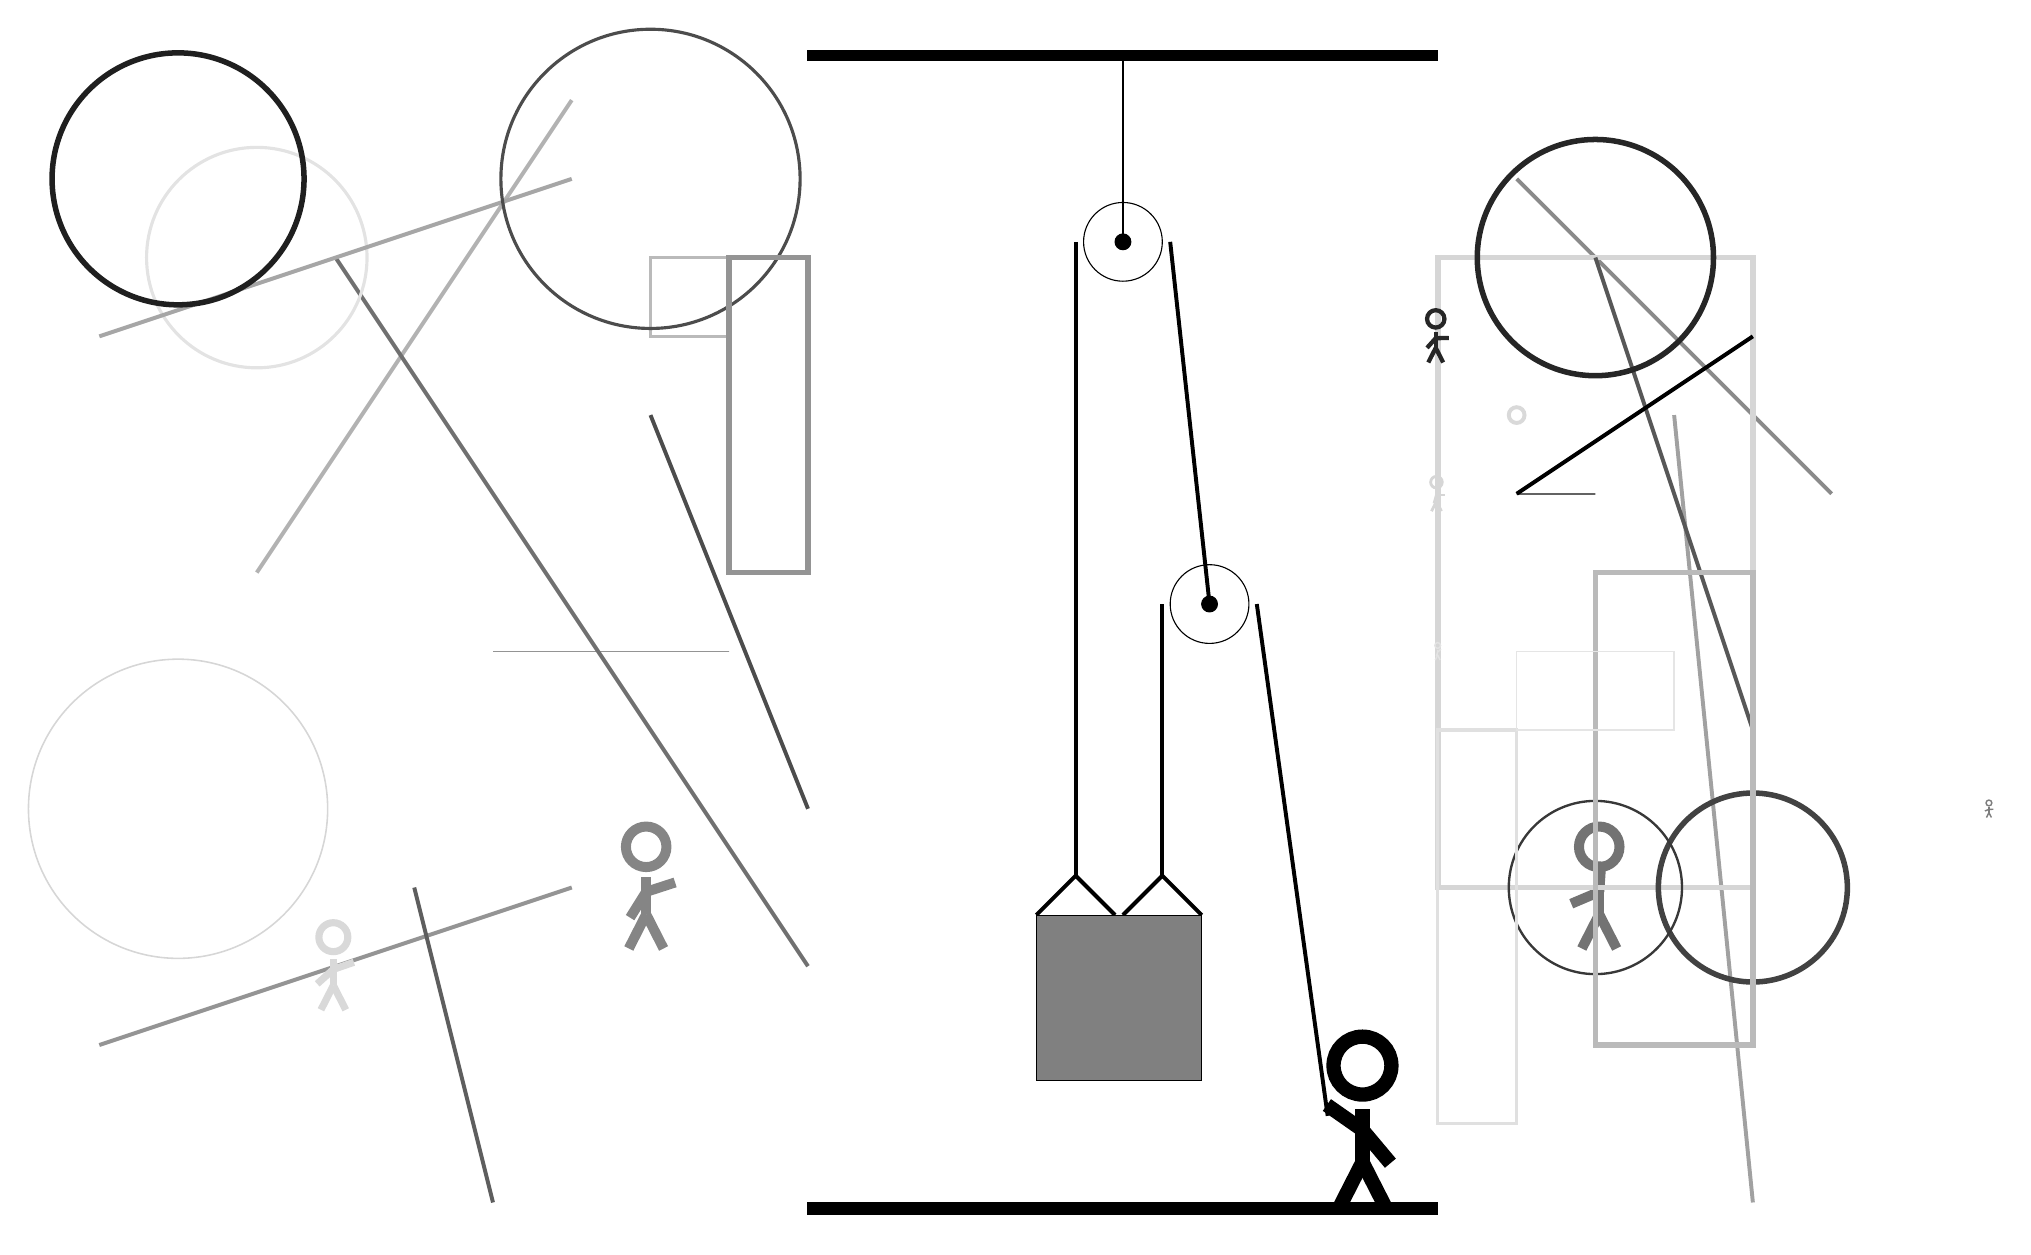
\begin{tikzpicture}
			%%%%% START %%%%%
			
			\draw[fill=black] (-2, 11.5) rectangle (6, 11.625);
			
			\draw (2, 9.2) circle (0.5);
			\draw[fill=black] (2, 9.2) circle (0.1);
			\draw[thick] (2, 9.2) -- (2, 11.5);
			
			\draw (3.1, 4.6) circle (0.5);
			\draw[fill=black] (3.1, 4.6) circle (0.1);
			
			\draw[line width = 0.5mm]  (0.9, 0.65) -- (1.4, 1.15) -- (1.9, 0.65);
			\draw[line width = 0.5mm]  (2.0, 0.65) -- (2.5, 1.15) -- (3.0, 0.65);
			\draw[fill=black!50] (0.9, 0.65) rectangle (3.0, -1.45);
			
			\draw[line width = 0.5mm] (1.4, 9.2) -- (1.4, 1.15);
			\centerarc[line width = 0.5mm](2, 9.2)(0:180:0.6);
			\draw[line width = 0.5mm] (2.6, 9.2) -- (3.1, 4.6);
			\draw[line width = 0.5mm] (2.5, 4.6) -- (2.5, 1.15);
			\centerarc[line width = 0.5mm](3.1, 4.6)(0:180:0.6);
			\draw[line width = 0.5mm] (3.7, 4.6) -- (4.6, -1.9);
			
			\node at (5, -2) {\Strichmaxerl[10][-35][-50]};
			
			\draw [line width=0.2mm, color=black!16](-10, 2) circle (1.9);
			
			\draw[line width=0.5mm, color=black!46](11, 6) -- (7, 10);
			\draw[line width=0.5mm, color=black!37](10, -3) -- (9, 7);
			\node[line width=0.4mm, color=black!16] at (6, 6) {\Strichmaxerl[2][74][0]};
			\draw[line width=0.5mm, color=black!30](-5, 11) -- (-9, 5);
			\draw[line width=0.2mm, color=black!42] (-3, 4) rectangle (-6, 4);
			\node[line width=0.7mm, color=black!55] at (8, 1) {\Strichmaxerl[7][23][86]};
			\draw[line width=0.7mm, color=black!16] (6, 9) rectangle (10, 1);
			\node[line width=0.5mm, color=black!48] at (-4, 1) {\Strichmaxerl[7][58][18]};
			\draw[line width=0.5mm, color=black!56](-2, 0) -- (-8, 9);
			
			\draw[line width=0.2mm, color=black!61] (7, 6) rectangle (8, 6);
			\draw [line width=0.4mm, color=black!11](-2, 2) circle (0.0);
			\node[line width=0.7mm, color=black!51] at (13, 2) {\Strichmaxerl[1][21][2]};
			
			\draw [line width=0.4mm, color=black!11](-9, 9) circle (1.4);
			\draw[line width=0.5mm, color=black!35](-5, 10) -- (-11, 8);
			\draw[line width=0.5mm, color=black!42](-5, 1) -- (-11, -1);
			\draw[line width=0.3mm, color=black!27] (-3, 8) rectangle (-4, 9);
			\draw[line width=0.5mm, color=black!66](10, 3) -- (8, 9);
			\draw [line width=0.7mm, color=black!74](10, 1) circle (1.2);
			\draw [line width=0.4mm, color=black!70](-4, 10) circle (1.9);
			\node[line width=0.5mm, color=black!15] at (-8, 0) {\Strichmaxerl[5][42][19]};
			\draw [line width=0.3mm, color=black!78](8, 1) circle (1.1);
			
			\draw [line width=0.5mm, color=black!15](7, 7) circle (0.1);
			\draw [line width=0.7mm, color=black!85](8, 9) circle (1.5);
			\node[line width=0.4mm, color=black!11] at (6, 4) {\Strichmaxerl[1][72][40]};
			
			\draw[line width=0.5mm, color=black!70](-2, 2) -- (-4, 7);
			
			\draw[line width=0.7mm, color=black!42] (-2, 5) rectangle (-3, 9);
			\draw [line width=0.7mm, color=black!88](-10, 10) circle (1.6);
			\draw[line width=0.5mm, color=black!100](7, 6) -- (10, 8);
			\draw[line width=0.4mm, color=black!12] (7, 3) rectangle (6, -2);
			\draw[line width=0.7mm, color=black!27] (8, -1) rectangle (10, 5);
			
			\node[line width=0.6mm, color=black!85] at (6, 8) {\Strichmaxerl[3][48][1]};
			\draw[line width=0.2mm, color=black!10] (7, 4) rectangle (9, 3);
			\draw[line width=0.5mm, color=black!63](-7, 1) -- (-6, -3);
			
			
			\draw[fill=black] (-2, -3) rectangle (6, -3.15);
			
			%%%%% END %%%%%
		\end{tikzpicture}
	\end{figure}	
\end{document}